\section{Motivation}

%{::comment}
%For this section I need to first provide motivation for concurrency, and define concurrency and parallelism. which are not commonly understood. Do I need to provide a motivation section for each chapter?
%{:/comment}

\textit{Concurrency} is when multiple tasks start, run, and complete in overlapping time periods and should not be confused with \textit{parallelism} which is when multiple tasks execute simultaneously. Parallelism requires some form of hardware support, where as concurrency can be achieved strictly through software, such as a cooperative tasking system.

There are two primary benefits for concurrent code. The first is performance by enabling parallelism. The second is to improve interactivity by not blocking the user while a prior action is being processed.

As clock rates on systems have stagnated, hardware developers have turned to parallelism to increase performance. Figure [xxx] shows the performance distribution on a typical desktop system. A single threaded, non-vectorized, application can only utilize about 0.25\% of the performance capabilities of the machine.

\section{Definition of \textit{raw synchronization primitives}}

A \textit{raw synchronization primitive} is a low level construct used to synchronize access to data. Examples include locks and mutexes, condition variables, semaphores, atomic operations, and memory fences.

\comment{Discuss difference between data parallelism and task concurrency, so far this chapter is only dealing with tasking. However, it could be expanded upon.}

The goal of this chapter is to develop concurrent code without using raw synchronization primitives.

The first problem with raw synchronization primitives are that they are exceedingly error prone to use because, by definition, they require reasoning about non-local effects.

For example, the following is a snippet from a copy-on-write data type, this is a simplified version of code from a shipping system. 

\begin{minipage}{\linewidth}
	\lstinputlisting[language=C++,
	                   %linebackgroundcolor={% }
	  ]{code/bad_cow.cpp}
\end{minipage}

\comment{highlight lines}
The highlighted lines contain a subtle race condition. The `if` statement at line 14 is checking the value of an atomic count to see if it is `1`. The `else` statement handles the case where it is not `1`. Within the else statement the count is decremented at line 17. The problem is that if decrementing the count results in a value of `0` then the object stored in `object\_m` should be deleted. The code fails to check for this case, and so an object may be leaked.

The initial test to see if the count was `1` isn't sufficient, between that check and when the count is decremented another thread may have released ownership and decremented the count leaving this object instance as the sole owner.

The fix is to test atomically with the decrement in the same statement, see line 17. The correct code is shown in shown below:

\begin{minipage}{\linewidth}
	\lstinputlisting[language=C++,
	                   %linebackgroundcolor={% }
	  ]{code/correct_cow.cpp}
\end{minipage}


\comment{Should we refer to the complete implementation?}
The code of the complete implementations is here\footnote{[https://github.com/stlab/libraries/blob/develop/stlab/copy\_on\_write.hpp](https://github.com/stlab/libraries/blob/develop/stlab/copy\_on\_write.hpp}

Another problem with raw synchronization primitives is that their use can have a large negative impact on system performance. To understand why, we need to understand Amdahl's Law.

The intuition behind Amdahl's Law is that if a part of system takes time x to complete on a single core or processor, then it will encounter a speedup of y if it is run on y cores, but only if no synchronization takes places between the different cores or processors. 

$$ S(N) = \frac{1}{(1-P)+\frac{P}{N}} $$
Where the speedup $S$ is defined by this equation. $P$ is hereby the amount of synchronization in the range of $[0 .. 1]$ and $N$ the number of cores or processors.

Drawing the abscissa in logarithmic scale illustrates that there is only a speedup of 20 times when the system is running on 2048 cores or more and just 5% synchronization takes place.

\begin{center}
  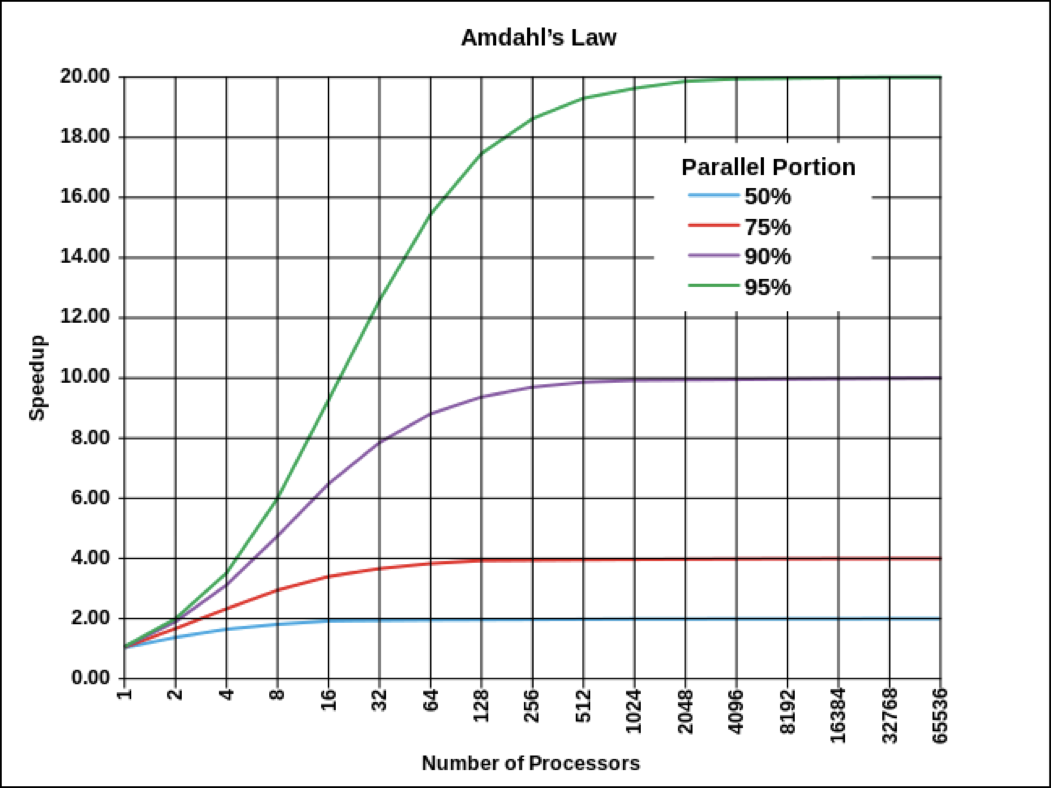
\includegraphics[width=0.5\textwidth]{images/amdahl_log.png}
\end{center}

Amdahl's Law Logarithmic Scale

\begin{center}
  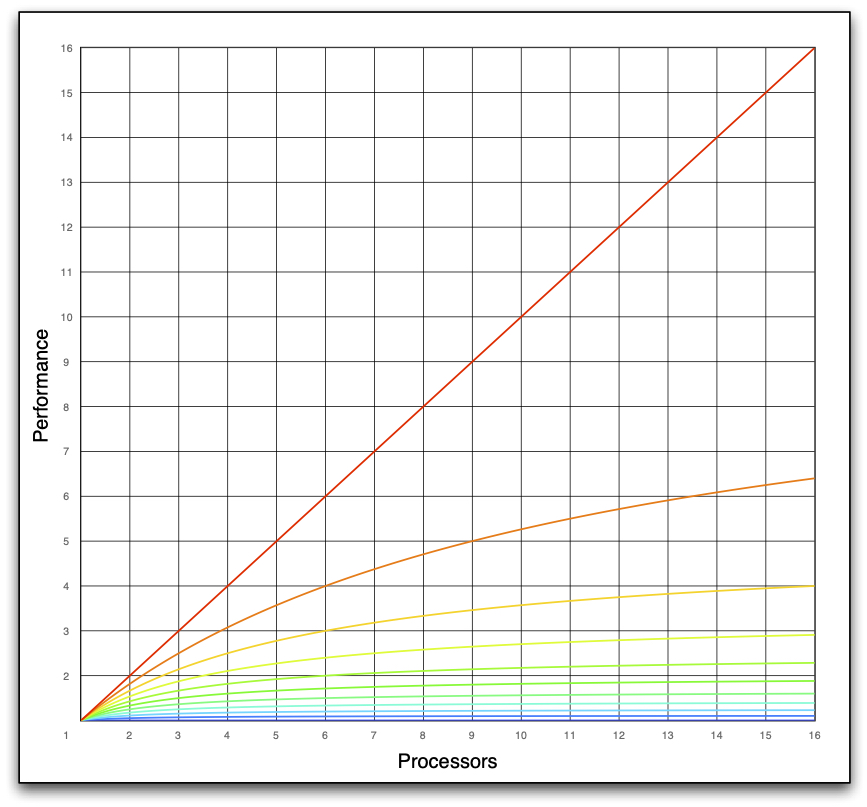
\includegraphics[width=0.5\textwidth]{images/amdahl_lin.png}
\end{center}

Amdahl's Law Linear Scale

Since most desktop or mobile processors have less than 64 cores, it is better to take a look at the graph with linear scale. Each line here represents just 10\% of serialisation. So if the application just have 10\% of serialisation and it is running on 16 cores then there is a speed-up just a little better than six times. 

So Amdahl's law has a huge impact. Serialization doesn't mean only locking on a mutex. Serialization can just mean sharing the same memory or sharing the same address bus for the memory if it is not a Numa architecture. Sharing the same cache line, anything that's shared within the processor starts to bend that curve down and it bends down rapidly, even an atomic bends that curve down.

An often used model for implementing exclusive access to an object by multiple threads is this:

\begin{table}[h!]
	\begin{tabular}{ c  c  c }
	  \begin{minipage}{.3\textwidth}
		  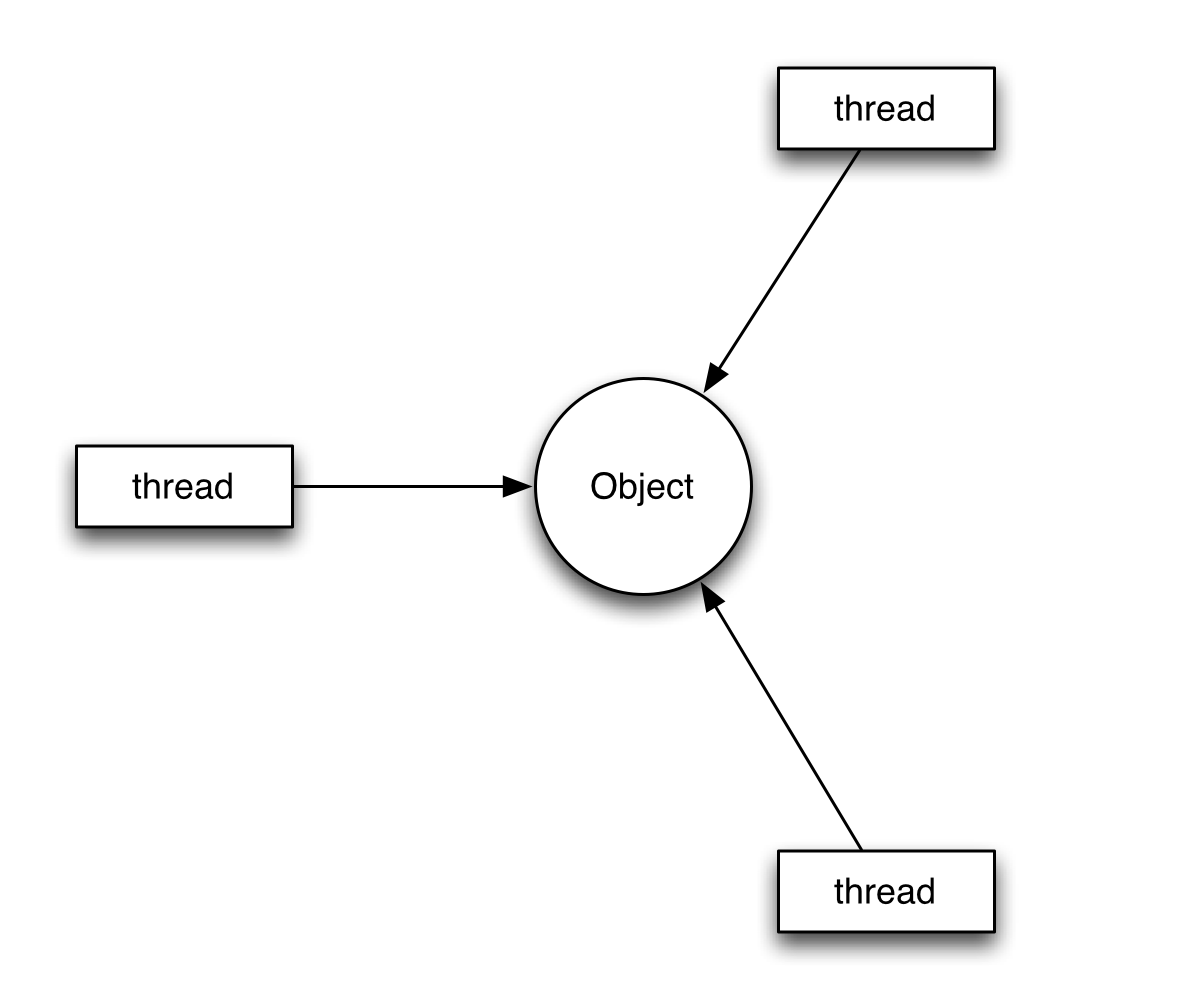
\includegraphics[width=\linewidth]{images/TraditionalLock01.png} 
		\end{minipage} 
		&
	  \begin{minipage}{.3\textwidth}
		  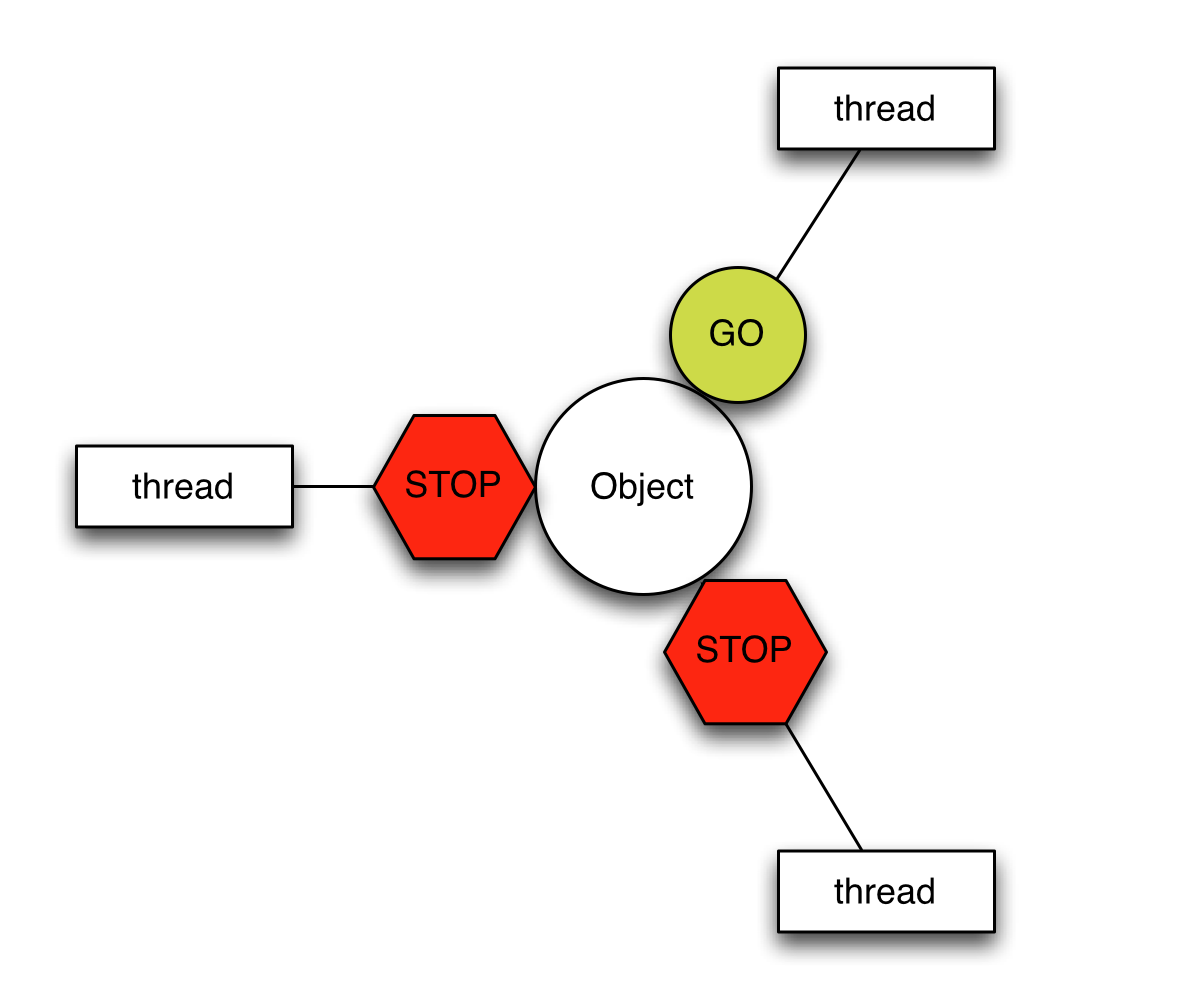
\includegraphics[width=\linewidth]{images/TraditionalLock02.png} 
		\end{minipage} 
		&
	  \begin{minipage}{.3\textwidth}
		  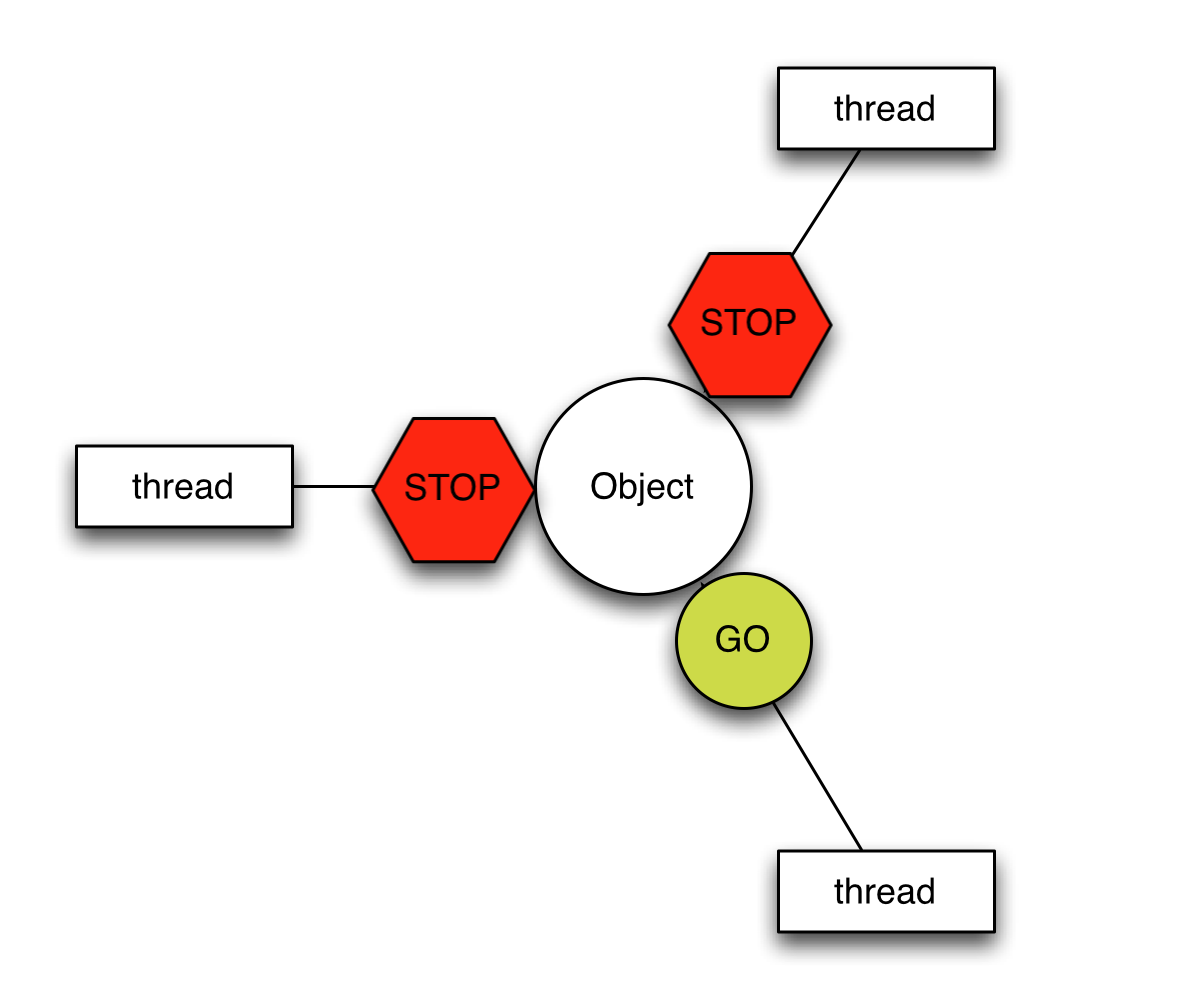
\includegraphics[width=\linewidth]{images/TraditionalLock03.png} 
		\end{minipage} 
	\end{tabular}
\end{table}

As long as one thread has exclusive access to the object all other threads have to wait until they get the access right. 

That is a horrible horrible way to think about threading. The goal has to be to minimize waiting at all costs. Because of this property of slowing down David Butenhof, one of the POSIX implementors coined the phrase that mutex should be better named bottleneck\footnote{http://zaval.org/resources/library/butenhof1.html}


So let's take a look at a traditional little piece of code here. 

\begin{minipage}{\linewidth}
	\lstinputlisting[language=C++,
	                   %linebackgroundcolor={% }
	  ]{code/registry-1.cpp}
\end{minipage}

%It is a registry class with shared set and a get functions where the access to the underlying unordered map is protected against concurrent access with a mutex. At the first glance it seems that only minimal work is done under the mutex. The unordered map is a fairly efficient data structure, it is a hash map. The amount of time it takes to hash the key depends on the length of the string. So the work that is being done under the lock here is actually fairly unbounded. It depends completely on the lengths of the string. It may be  probably typically small but it could be big. On top of calculating the hash comes a potentially allocation of a new bucket within the unordered map, which in most cases requires another lock within the memory manager.
%
%For a better understanding what shall be actually achieved by using the locks it is necessary to take step back. The C++ standard states here: _It can be shown that programs that correctly use mutexes and memory\_order\_seq\_cst operations to prevent all data races and use no other synchronization operations behave as if the operations executed by their constituent threads were simply interleaved, with each value computation of an object being taken from the last side effect on that object in that interleaving. This is normally referred to as ‘sequential consistency.’, C++11 Standard 1.10.21.
%
%So why is this an important sentence? It means that one can always think about mutexes as if one has some set of interleaved operations. 
%
%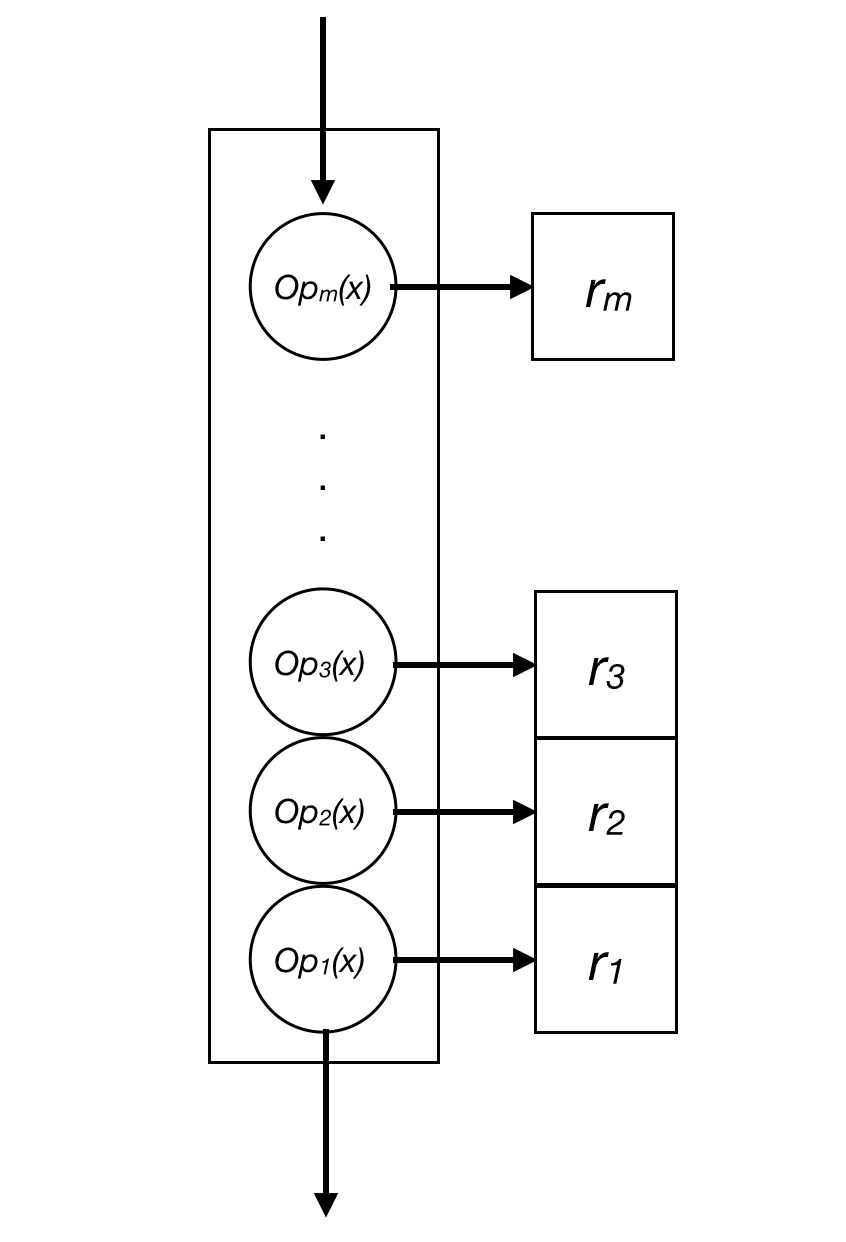
\includegraphics[width=0.25\textwidth]{images/SequentialOperations.png)}
%
%that we have op so I can have operation 3 repeated multiple times. and and what an operation is is that's the code that's executing onto the lock and its operating on some value what's that value it's the set of all objects that are modified by all operations. okay so so X is everything that gets modified within my lock ok by all the pieces of code that acquire that lock on the mutex ok and each of those can yield out some values some result right those operations can say it's a read-modify-write operation they can read modify write the data under that yielding out some results from the read okay 
%
%\begin{itemize}
%\item A mutex serializes a set of operations, Opn, where the operation is the code executed while the mutex is locked
%\item Operations are interleaved and may be executed in any order and may be repeated
%\item Each operation takes an argument, X, which is the set of all objects mutated under all operations
%	\begin{itemize}
%	\item X may not be safely read or written without holding the lock if it may be modified by a task holding the lock
%	\end{itemize}
%\item Each operation may yield a result, rm, which can communicate information about the state of X while it’s associated operation was executed
%
%\item The same is true of all atomic operations
%\end{itemize}
%
%
%
%
%
%
%%so the same is true of all atomic operations right so there's really not a lot of difference between an STD atomic in fact there is a call on STD atomic that says is this lock free so what that means is is their processor support to do that as an atomic item within the processor or is there not processor support and the compiler has to generate a mutex pair to to lock make the change on the atomic operation and do the the unlock right so all that mutexes and locks are our way to construct atomic operations right 
%
%
%
%So if you look you know fetch subtract follows from my previous example for the bad cow you're doing a section subtract that's a read modify write operation on X to the atomic 
%
%So one can take any piece of code that has mutexes and transform it into a queued model:
%\lstinputlisting[language=C++,
%                   %linebackgroundcolor={% }
%  ]{code/registry-2.cpp}

%Under the assumption that one has a serial queue `_q` and my serial q has just one operation on it which is go a sync execute this thing and it's the same same calling conventions as STD async here except it guarantees that that the next item being processed in that queue doesn't start until the previous one completed okay then I can rewrite my set string to go do QA sync okay and I can rewrite my get string but I've got a little bit of a problem there in that I need the result back out and I need it paired with that particular gift okay so I'm going to use a future there and we'll talk more about futures okay and I've got the Q async here why is this important to understand because any place I have a mutex in my code I can always make this transformation I can always trance form it into a serialize queue model and that means that within the serialized queue model now anytime somebody comes along and says set here regardless of the amount of work that set takes the time it takes for set to return back to the caller is constant okay so that means that I can add something like set an arbitrary set of value the whole vector of key value pairs okay and to the caller that set will take just as much time as the previous set it's an on block okay so so this puts an upper bound now there's overhead in this right I've got to queue an item I've got to DQ the item I've got to deal with futures if I've got results coming in if I'm calling this set as opposed to calling just set string set sync set string

\section{Develop Solution}

\section{Conclusion}
